\documentclass[tikz,border=6pt]{standalone}
\usepackage[T1]{fontenc}
\begin{document}
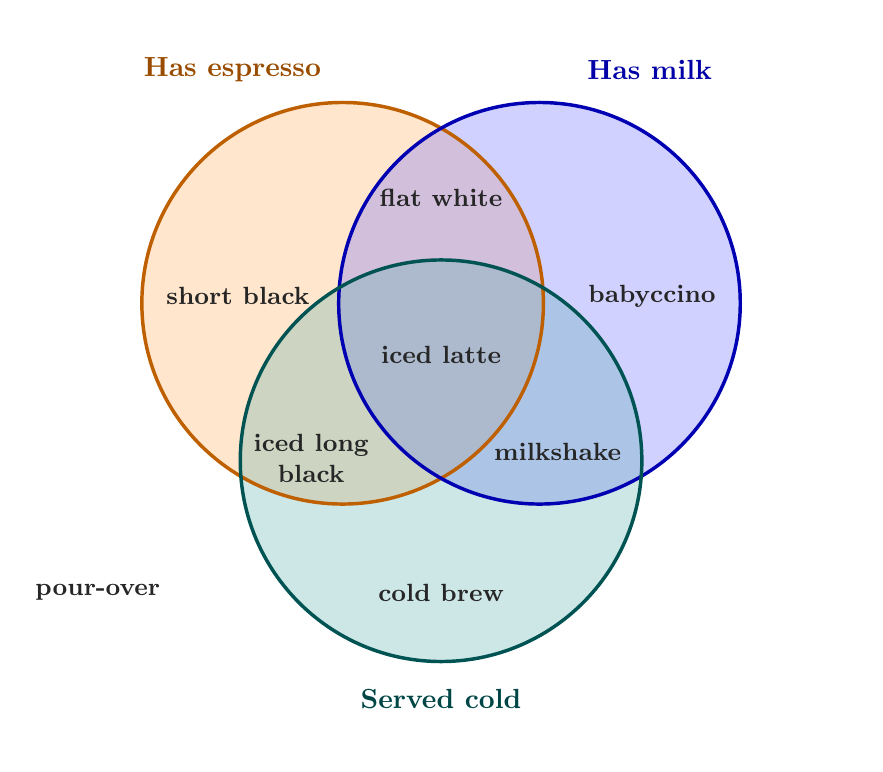
\begin{tikzpicture}[font=\sffamily]
  \path[use as bounding box] (-5.25,-4.65) rectangle (5.25,4.45);

  % Three translucent sets; draw the outlines on top of all the fills.
  \fill[orange!65,opacity=.30] (-1.25,.95) circle (2.55);
  \fill[blue!60,opacity=.30] (1.25,.95) circle (2.55);
  \fill[teal!65,opacity=.30] (0,-1.05) circle (2.55);
  \draw[orange!75!black,line width=1.25pt] (-1.25,.95) circle (2.55);
  \draw[blue!70!black,line width=1.25pt] (1.25,.95) circle (2.55);
  \draw[teal!65!black,line width=1.25pt] (0,-1.05) circle (2.55);

  \node[font=\bfseries, text=orange!60!black] at (-2.65,3.91) {Has espresso};
  \node[font=\bfseries, text=blue!65!black] at (2.65,3.91) {Has milk};
  \node[font=\bfseries, text=teal!55!black] at (0,-4.07) {Served cold};

  \tikzset{drink/.style={align=center,font=\small\bfseries,text=black!85}}
  \node[drink] at (-2.58,1.04) {short black};
  \node[drink] at (2.68,1.04) {babyccino};
  \node[drink] at (0,2.29) {flat white};
  \node[drink] at (-1.65,-1.02) {iced long\\black};
  \node[drink] at (1.48,-.94) {milkshake};
  \node[drink] at (0,.29) {iced latte};
  \node[drink] at (0,-2.73) {cold brew};
  \node[drink] at (-4.36,-2.72) {pour-over};
\end{tikzpicture}
\end{document}
